\documentclass[uplatex,dvipdfmx]{jlreq}
\usepackage[fleqn,tbtags]{mathtools}
\usepackage{jlreq-deluxe}
\usepackage{geometry}
\usepackage{booktabs}
\usepackage{hyperref}
\usepackage[noalphabet]{pxchfon} % must be after otf package
\usepackage{stix2} %欧文＆数式フォント
\usepackage[fleqn,tbtags]{mathtools} % 数式関連 (w/ amsmath)
\usepackage{url}
\usepackage{here}
\geometry{left=20mm,right=20mm,top=25mm,bottom=25mm}

\title{作業ログ\\ \large 加速度センサーを用いた身体動作による輪唱制御システムの構築と視覚フィードバック効果}
\author{報告者: 早川　和輝}
\date{報告日: 2026年7月8日}

\begin{document}
\maketitle

\section{進捗サマリー(要約)}
\begin{itemize}
    \item 全体進捗率: [98\%]
    \item マイルストーン達成状況: [達成]
    \item 主要成果:
    \begin{itemize}
        \item 成果1: LEDマトリクスのカエル図案(3コマアニメ)を再作成し，大きな目・鼻の穴・にっこり口・4本足を備えたカエルらしい見た目へ改善した．
        \item 成果2: サーボモーターに取り付ける可動部を作成．土台に固定したサーボへ割り箸をくくりつけ，その割り箸にカエルの折り紙を貼り付けて，跳ねるように動く機構を構成した．
        \item 成果3: マトリクスのカエル表示・サーボ駆動・音を合わせた結合テストを実施し，成功した．
    \end{itemize}
    \item 重大課題(影響度:無し): なし
\end{itemize}

\section{作業ログ(詳細トラッキング)}
\begin{table}[H]
    \centering
    \small
    \begin{tabular}{lp{1.5cm}p{1.5cm}llp{2.5cm}p{3cm}}
        \toprule
        作業項目 & 開始日 & 完了日 & 状態 & 進捗率 & 依存関係・ブロッカー & コメント \\
        \midrule
        マトリクスのカエル再作成 & [7/1] & [7/3] & 完了 & 100\% & なし & LEDマトリクスのカエルのドット絵を描き直し，目・鼻・口・4本足を備えたカエルらしい3コマアニメへ改善． \\
        サーボ可動部の作成 & [7/2] & [7/5] & 完了 & 100\% & なし & 土台に固定したサーボへ割り箸をくくりつけ，割り箸にカエルの折り紙を貼付．跳ねる動きを構成． \\
        結合テスト & [7/4] & [7/7] & 完了 & 100\% & サーボ可動部・マトリクス再作成 & マトリクス表示・サーボ駆動・音を合わせて動作確認．結合テストは成功． \\
        \bottomrule
    \end{tabular}
\end{table}

\section{担当箇所の計画前のGCと現在のGC}
担当箇所である「楽器演奏実装」および「視覚フィードバック(カエルの表示・可動部)」における，当初計画時（計画前）のガントチャート（GC）の予定と，現在の進捗・変更状況の比較である．
\begin{table}[H]
    \centering
    \small
    \begin{tabular}{lp{4cm}p{4cm}l}
        \toprule
        タスク名 & 計画前のGC（予定期間） & 現在のGC（実績・修正期間） & 進捗状態 \\
        \midrule
        マトリクスのカエル再作成 & [6/30 $\sim$ 7/3] & [7/1 $\sim$ 7/3] & 完了 \\
        サーボ可動部の作成 & [7/1 $\sim$ 7/5] & [7/2 $\sim$ 7/5] & 完了 \\
        結合テスト & [7/4 $\sim$ 7/7] & [7/4 $\sim$ 7/7] & 完了 \\
        \bottomrule
    \end{tabular}
\end{table}\begin{figure}[H]
    \centering
    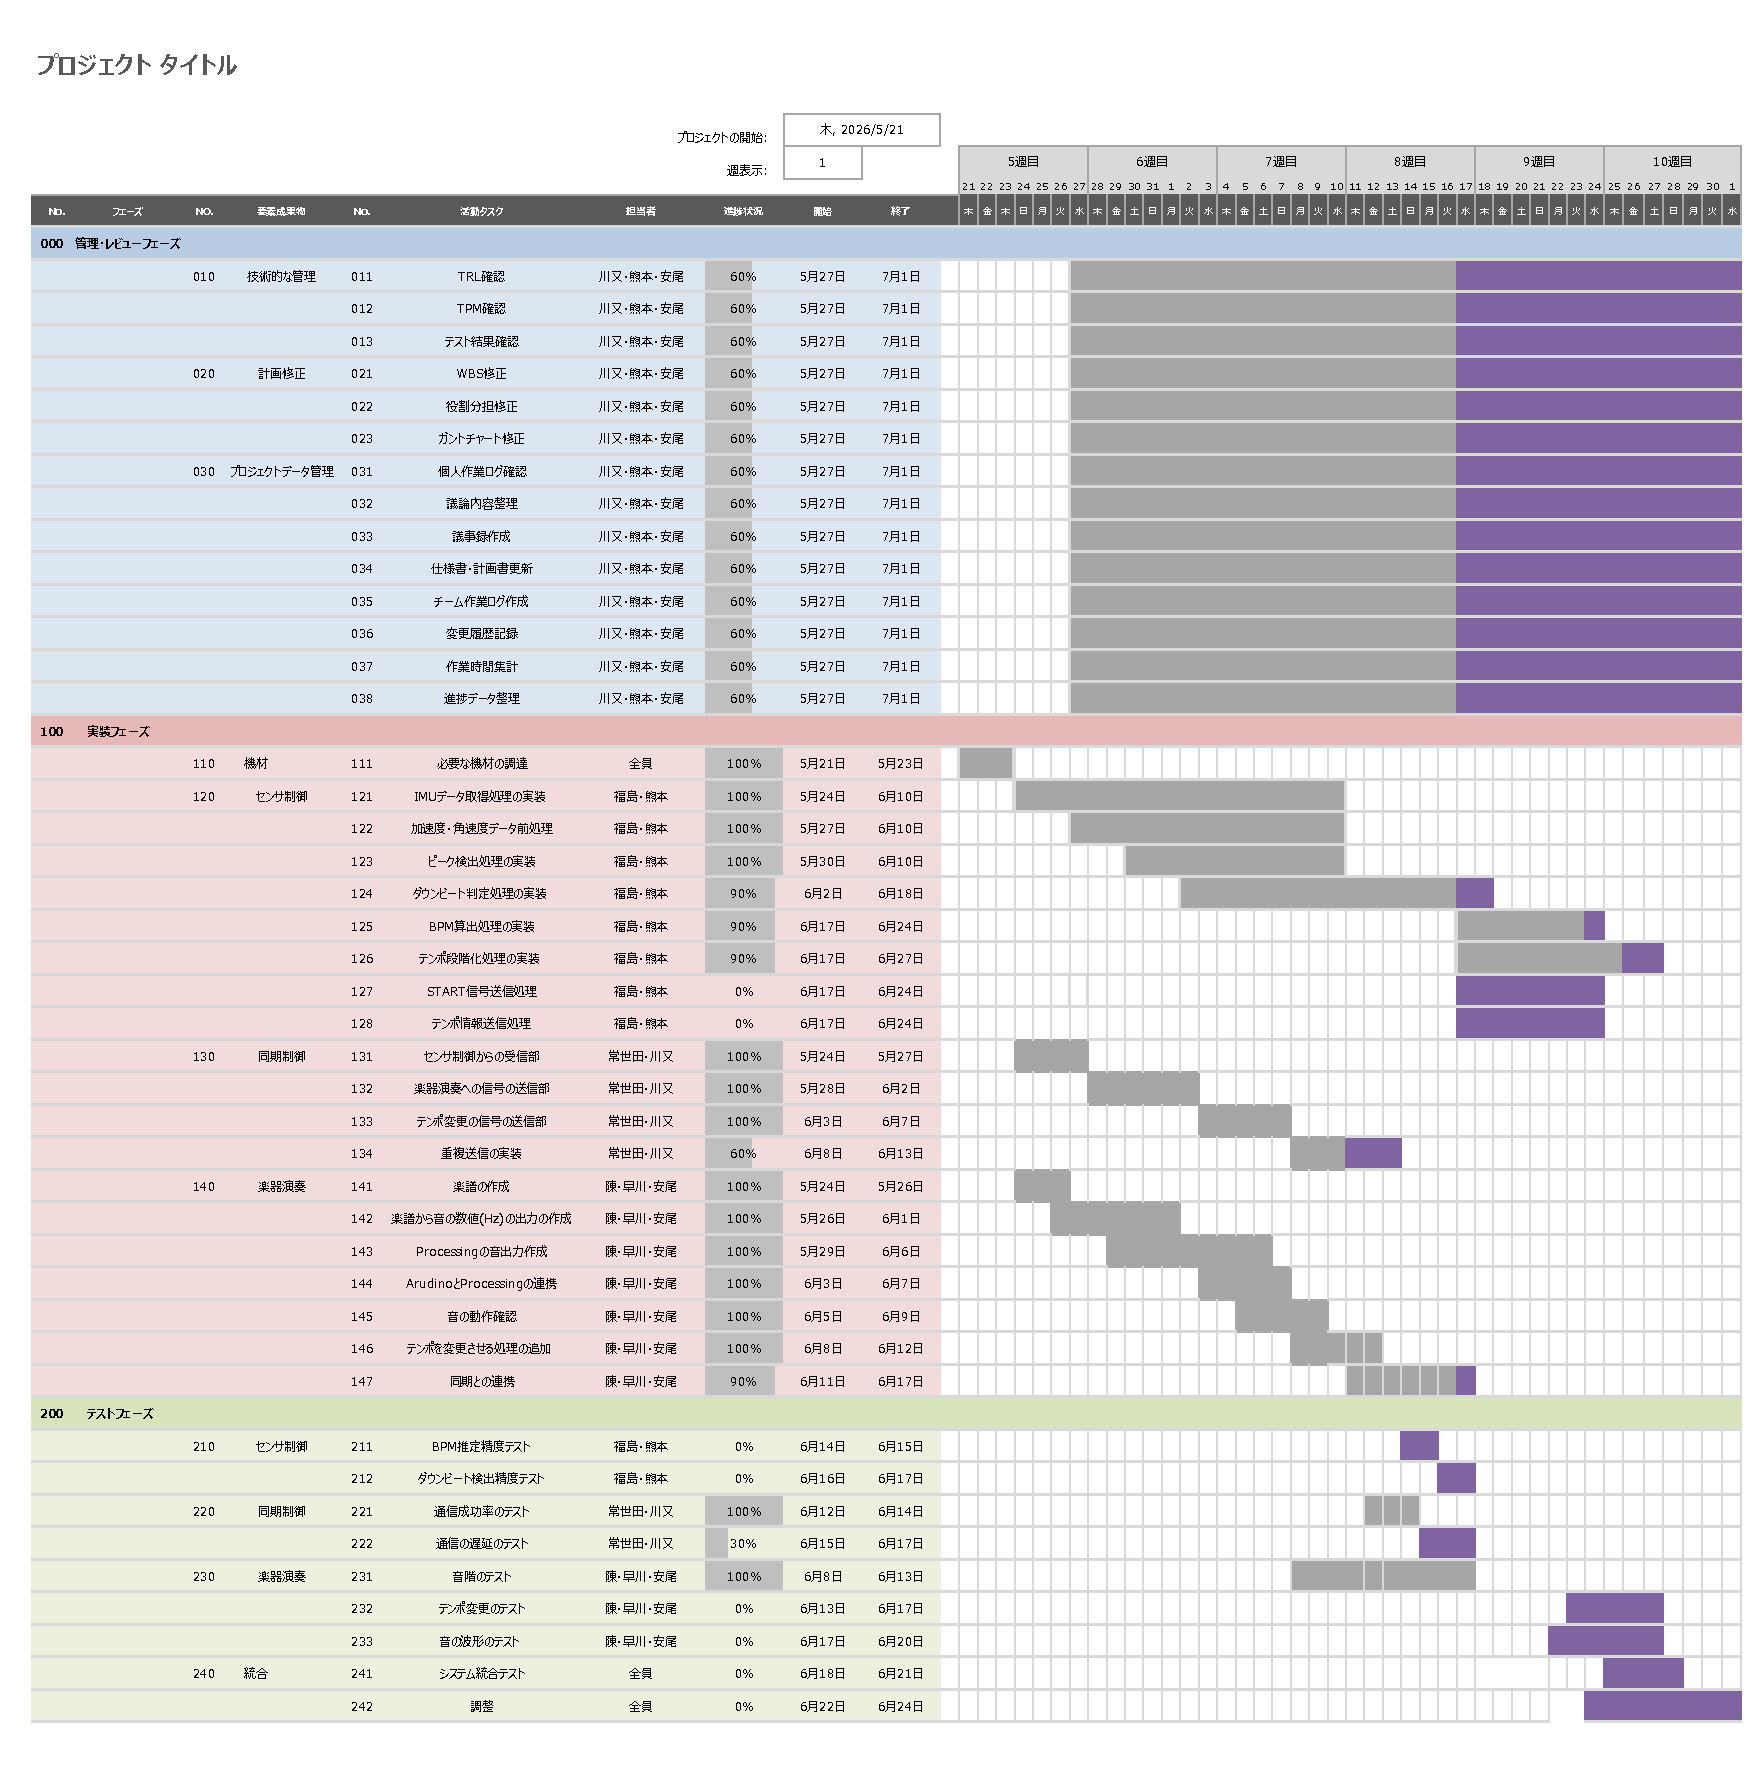
\includegraphics[width=0.8\textwidth]{gant8.pdf}
    \caption{ガントチャート}
\end{figure}

\section{日ごとの作業時間と作業内容}
今週実施した日ごとの具体的な作業時間および対応内容の詳細です．
\begin{table}[H]
    \centering
    \small
    \begin{tabular}{lll}
        \toprule
        日付 & 作業時間 & 作業内容 \\
        \midrule
        {}[7/1] & [2.0時間] & LEDマトリクスのカエル図案(3コマアニメ)の再作成と表示確認． \\
        {}[7/4] & [2.0時間] & サーボへ割り箸をくくりつけ，割り箸にカエルの折り紙を貼付する可動部の作成． \\
        {}[7/7] & [2.0時間] & マトリクス表示・サーボ駆動・音を合わせた結合テスト(成功)． \\
        \midrule
        \textbf{合計} & \textbf{[6.0時間]} & \\
        \bottomrule
    \end{tabular}
\end{table}

\section{課題管理}
\begin{table}[H]
    \centering
    \small
    \begin{tabular}{p{3cm}p{3cm}llp{3cm}ll}
        \toprule
        課題 & 発生原因 & 影響度 & 優先度 & 対策 & 期限 & 状態 \\
        \midrule
        マトリクス図案の視認性 & 旧図案が塊状でカエルに見えにくかった & 低 & 中 & 目・鼻・口・4本足を明確化したドット絵へ再設計し，実機で視認性を確認 & [7/3] & 解決 \\
        可動部のぐらつき・揺れ & 割り箸の固定やカエル折り紙の重さでサーボ動作時に揺れる可能性 & 中 & 中 & くくりつけ位置と貼付位置を調整し，安定して跳ねる動きを確認 & [7/5] & 解決 \\
        結合時の動作整合 & マトリクス・サーボ・音を同時駆動した際の動作確認が未実施 & 中 & 高 & 結合テストを実施し，各要素が問題なく連動することを確認(成功) & [7/7] & 解決 \\
        \bottomrule
    \end{tabular}
\end{table}
\vspace{0.5em}
\noindent ※影響度=プロジェクトへのインパクト，優先度=対応の緊急性

\section{AI 利用状況と検証(再現性重視)}
\subsection{利用内容}
\begin{itemize}
    \item 利用目的: LEDマトリクスに表示するカエルのドット絵(3コマアニメ)の再作成
    \item  入力(プロンプト要旨):
    \begin{itemize}
        \item よりカエルらしく見えるよう，マトリクスのカエル図案の描き直しを依頼．
    \end{itemize}
    \item  出力概要:
    \begin{itemize}
        \item 大きな目・鼻の穴・にっこり口・4本足を備えたカエルの3コマ分ビットマップ(FrogMatrix.h)．
    \end{itemize}
\end{itemize}

\subsection{検証方法}
\begin{itemize}
    \item  検証手法: 生成されたビットマップのASCIIプレビュー確認および実機マトリクスでの表示確認
    \item  参照資料: 従来のFrogMatrix.hおよびカエルの見た目の要件
    \item  検証手順:
    \begin{enumerate}
        \item 各コマのドット配置をASCIIで可視化し，カエルの目・鼻・口・足が意図通りに描けているか目視で確認．
        \item 実機のLEDマトリクスへ書き込み，3コマアニメがカエルらしく表示されることを確認．
    \end{enumerate}
\end{itemize}

\section{その他}
サーボに取り付けた割り箸とカエルの折り紙による可動部を，マトリクス表示・音と合わせた結合テストで確認し，成功した．

\end{document}
